\chapter{Methodology}
% TODO: overview of the chapter





%%%%%%%%%%%%%%%
\section{System architecture}
\label{sec:SystemArchitecture}
As depicted in figure \ref{fig:pa:systemBlockDiagram}, we use the pose estimates calculated using stereo images and \gls{LiDAR} point clouds as relative measurements. ORB SLAM 2 and LegoLOAM algorithms, respectively, are used for this purpose. Furthermore, \gls{GNSS} measurements and orientation estimated from magnetometer measurements act as positional and rotational absolute measurements to the fusion mechanism. The fusion mechanism is an \gls{ES-EKF} with 16 variables in the state space and 15 variables in the error state space. The output of the system consists of a state vector including position, orientation and velocity of the vehicle relative to a global frame of reference. Estimated covariance of the error is also provided, from which, the 99\% confidence interval ($3\sigma$ bound) can be derived. Output is compared with the ground truth provided with the dataset being used, to calculate the resultant error margins.
\begin{figure}[h]
	\begin{center}
	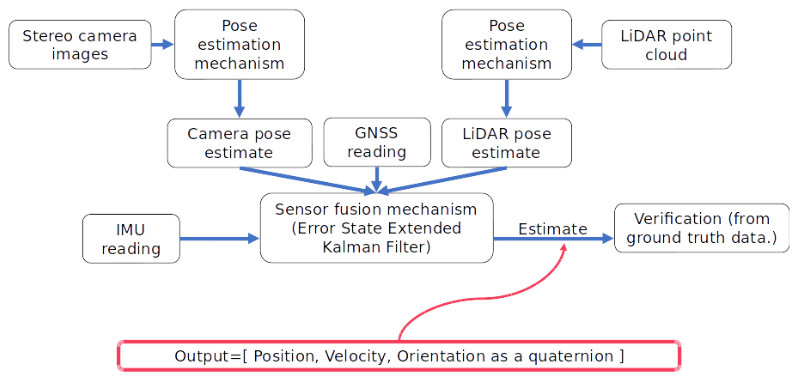
\includegraphics[width=\textwidth]{figs/system-block-diagram.png}
	\end{center}
	\vspace{-0.5cm}
	\caption{System block diagram}
	\label{fig:pa:systemBlockDiagram}
	\vspace{0.5cm}
\end{figure}

The system is implemented on \gls{ROS}, along with evaluation and visualization mechanisms for demonstrating functionality. Main programming language used is Python. Each of the components mentioned in the above discussion will be explained in detail, in the subsequent sections.







%%%%%%%%%%%%%%%
\section{Coordinate frames}
Apart from each sensor's own coordinate frame, in which they provide measurements, we define the following coordinate frames which will be used in the rest of this report.\\\\
\begin{tabular}{p{0.2\linewidth} p{0.75\linewidth} } 
	Inertial frame & An earth fixed right-handed rectilinear coordinate frame with x, y and z axes pointing towards East, North and Up directions respectively(ENU frame). The origin of the frame is determined by the information given in the dataset being used.\\\\
	Body frame & A right-handed rectilinear coordinate frame fixed to the vehicle with x, y and z directions pointing lateral, front and upward directions of the vehicle respectively.
\end{tabular}\\\\
Figure \ref{fig:pa:coordinateFrames} illustrates the above-mentioned coordinate frames.
\begin{figure}[h]
	\begin{center}
	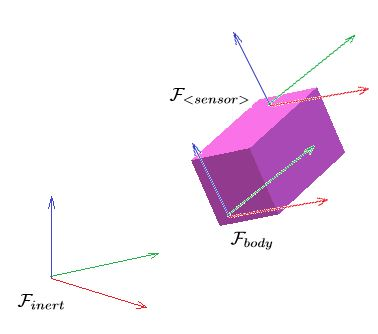
\includegraphics[width=0.6\textwidth]{figs/coordinate-frames.jpg}
	\end{center}
	\vspace{-0.5cm}
	\caption[Coordinate frames]{Illustration of the coordinate frames. x, y and z axes of each coordinate frame is depicted in red, green and blue colours, respectively. The cuboid represents the vehicle. The sensor is assumed to be mounted on the front side of the roof of the vehicle.}
	\label{fig:pa:coordinateFrames}
	\vspace{0.5cm}
\end{figure}







%%%%%%%%%%%%%%%
\section{Sensor fusion mechanism}
\subsection{The \acrlong{ES-EKF}}
The \gls{ES-EKF} acts as the component responsible for fusing sensor data. As mentioned in section \ref{sec:SystemArchitecture}, our \gls{ES-EKF} currently has 16 nominal state space variables and 15 error state space variables, grouped into 5 sub-vectors, as listed below;
\begin{align}
    \text{Nominal state vector: }\textbf{x} &= \left[\begin{matrix}{}\textbf{p}\\\textbf{v}\\\textbf{q}\\\boldsymbol{a_b}\\\boldsymbol{\omega_b}\end{matrix}\right]
\end{align}
where
\begin{align}
    \textbf{p} &= (p_x, p_y, p_z) \text{ position relative to the inertial frame} \nonumber \\
    \textbf{v} &= (v_x, v_y, v_z) \text{ velocity relative to the inertial frame} \nonumber \\
    \textbf{q} &= (q_w, q_x, q_y, q_z) \text{ quaternion relative to the inertial frame} \nonumber \\
    \boldsymbol{a_b} &= (a_{bx}, a_{by}, a_{bz}) \text{ acceleration biases of the IMU relative to the body frame} \nonumber \\
    \boldsymbol{\omega_b} &= (\omega_{bx}, \omega_{by}, \omega_{bz}) \text{ angular velocity biases of the IMU relative to the body frame}
\end{align}
and
\begin{align}
	\text{Error state vector: }\boldsymbol{\delta}\textbf{x} &= \left[\begin{matrix}{}\boldsymbol{\delta}\textbf{p}\\\boldsymbol{\delta}\textbf{v}\\\boldsymbol{\delta}\boldsymbol{\theta}\\\boldsymbol{\delta}\boldsymbol{a_b}\\\boldsymbol{\delta}\boldsymbol{\omega_b}\end{matrix}\right].
\end{align}
Here, $\boldsymbol{\delta}\boldsymbol{\theta}$ is the error in orientation, expressed as an axis-angle vector. Furthermore, $\boldsymbol{\delta}\boldsymbol{a_b}$ and $\boldsymbol{\delta}\boldsymbol{\omega_b}$ are the considered as global errors. The motion model for the prediction step of the filter is given below.\\
Nominal state update:
\begin{align}
    \check{\textbf{p}}_k &= \hat{\textbf{p}}_{k-1}+\hat{\textbf{v}}_{k-1}\Delta t + \frac{1}{2} \left( \textbf{R}_{inert,body}\left(\textbf{a}_{m_{k-1}}-\hat{\textbf{a}}_{b_{k-1}}\right)+\textbf{g}\right)\Delta t^2 \\
    \check{\textbf{v}}_k &= \hat{\textbf{v}}_{k-1}+\left(\textbf{R}_{inert,body}\left(\textbf{a}_{m_{k-1}}-\hat{\textbf{a}}_{b_{k-1}}\right)+\textbf{g}\right)\Delta t \\
    \check{\textbf{q}}_k &= \hat{\textbf{q}}_{k-1}\otimes \textbf{q}\left\{\left(\boldsymbol{\omega}_{m_{k-1}}-\hat{\boldsymbol{\omega}}_{b_{k-1}}\right)\Delta t\right\} \\
    \check{\textbf{a}}_{b_k} &= \hat{\textbf{a}}_{b_{k-1}} \\
    \check{\boldsymbol{\omega}}_{b_{k}} &= \hat{\boldsymbol{\omega}}_{b_{k-1}}
\end{align}
with
\begin{align}
	\textbf{a}_{m_{k}} &= \text{Acceleration measured by accelerometer at k\textsuperscript{th} instance}\\
	\boldsymbol{\omega}_{m_{k}} &= \text{Angular velocity measured by gyroscope at k\textsuperscript{th} instance}\\
    \textbf{R}_{inert,body} &= \text{Rotation matrix corresponding to $\hat{\textbf{q}}_{k-1}$} \\
	\textbf{g} &= \text{Gravity vector w.r.t inertial frame}\\
	\otimes &= \text{Quaternion composition operator.}
\end{align}
Error state covariance matrix update:
\begin{align}
    \Check{\textbf{P}}_k &= \textbf{F}_x\hat{\textbf{P}}_{k-1}\textbf{F}_x^T + \textbf{F}_i\textbf{Q}_i\textbf{F}_i^T
\end{align}
where
\begin{align}
	\textbf{P}_k &= \text{Error state covariance matrix at k\textsuperscript{th} instance}\\
	\textbf{F}_x &= \left.\frac{\partial f}{\partial \boldsymbol{\delta}\textbf{x}}\right|_{\textbf{x}=\hat{\textbf{x}}_{k-1} , \boldsymbol{\delta}\textbf{x}=\textbf{0} , \textbf{w}=\textbf{0}}\\
	\textbf{F}_i &= \left.\frac{\partial f}{\partial \textbf{w}}\right|_{\textbf{x}=\hat{\textbf{x}}_{k-1} , \boldsymbol{\delta}\textbf{x}=\textbf{0} , \textbf{w}=\textbf{0}}\\
	f(.) &= \text{Function representing the motion model}\\
	\textbf{w} &= \text{Process noise vector}\\
	\textbf{Q}_i &= \text{Process noise covariance matrix}.
\end{align}
The equations pertaining to the correction process, upon receiving a measurement update is given below.
\begin{align}
    \textbf{K}_k &= \check{\textbf{P}}_k\textbf{H}^T\left(\textbf{H}\check{\textbf{P}}_k\textbf{H}^T+\textbf{V}\right)^{-1} \\
    \hat{\textbf{P}}_k &= \left(\textbf{I}-\textbf{K}_k\textbf{H}\right)\check{\textbf{P}}_k\\
	\hat{\boldsymbol{\delta}\textbf{x}_k} &= \textbf{K}_k \left(\textbf{y}-h\left(\check{\textbf{x}}_k\right)\right)\\
	\hat{\textbf{x}}_k &= \check{\textbf{x}}_k \oplus \hat{\boldsymbol{\delta}\textbf{x}}_k\\
	\hat{\boldsymbol{\delta}\textbf{x}}_k & \leftarrow \textbf{0}.
\end{align}
Here,
\begin{align}
	h(.) &= \text{Measurement function}\\
	\textbf{H} &= \text{Jacobian of the measurement function, relative to the error state,}\nonumber\\
	&\quad\text{ evaluated at zero}\\
	\textbf{V} &= \text{Measurement noise matrix}\\
	\textbf{y} &= \text{Measurement vector}\\
	\textbf{I} &= \text{Identity matrix of suitable dimension}\\
	\oplus &= \text{Operator representing the combination of nominal state and error state }\nonumber\\
	&\quad\text{ vectors}.
\end{align}
For a detailed presentation of the matrices included in above equations, refer Appendix \ref{appendix:ESEKFMatrices}\cite{pa:Sola2017QuaternionKinematics}.


\subsection{Stochastic cloning and backward smoothing}
Following the works of Emter et. al\cite{pa:Emter2018StochasticCloning},  we have implemented a stochastic cloning framework along with the \gls{ES-EKF}, as a mean of integrating relative measurements obtained from sensors such as wheel odometer and visual/\gls{LiDAR} odometry algorithms. Since a relative measurement relates the current state of the vehicle to a previous state, it is required to propagate the corrections resultant from absolute measurements to all the previous states as well. In-order to achieve this, a \gls{RTS} backward smoother was integrated.


\subsection{State buffer}
It is essential to store a window of previous estimates obtained as the output of the \gls{ES-EKF}, in-order to be used when fusing a relative measurement, under stochastic cloning framework. A buffer with predefined length was implemented to achieve this functionality. Once a prediction is done by the \gls{ES-EKF}, the estimate is added to the buffer. If the buffer is full, the oldest estimate will be removed, keeping the buffer length a constant.

Other than the estimate itself, the motion model inputs that resulted the prediction of the estimate and the prediction covariance matrix are also stored in this buffer. In addition to the stochastic cloning mechanism, they are used in propagating the effect of an absolute measurement correction across all the states of the buffer.

\subsection{Time synchronization}
Measurements from different sensors arrive at different times, in different rates. These asynchronous arrivals are handled using the \gls{ROS}'s in-built multi-threading behaviour of subscriber callback functions. Each sensor publishes data to its own \gls{ROS} topic, for which the localization module is subscribed to. Hence, each publication will invoke a callback function, which includes the logic for carrying out either a prediction or a correction step, depending on the measurement received.

When an absolute correction is to be carried out, the filter first searches the state buffer, for the state with the closest timestamp to that of the measurement. Then it performs correction steps on that state. After it has been completed, the effect of the correction has to be propagated to all the remaining states in the buffer. States having later timestamps will be adjusted by re-predicting them based on the corrected state. States with earlier timestamps will be adjusted through performing \gls{RTS} smoothing. A similar procedure is carried out upon receiving a relative measurement, except that, backward smoothing with \gls{RTS} will not be performed.

In this manner, a delayed measurement can still contribute to a correction, unless it is too delayed, so that the state corresponding to its timestamp no longer exists in the state buffer.

If a prediction is to be carried out, the filter will only search for the latest timestamp of the states. If it is greater than that of the prediction input, the input will be neglected. Otherwise, a prediction will be carried out and the newly predicted state will be added to the state buffer.

% TODO: add image illustrating time synchronization


\subsection{\acrlong{ZUPT} measurements}
Some of the physical constraints that govern the motion of a vehicle can be incorporated into the sensor fusion mechanism, in-order to make the estimate more accurate. \gls{ZUPT} measurements, generated based on the fact that the motion of a vehicle is constrained only towards its longitudinal direction, are one such constraint that can be employed to couple the positional measurements with the heading estimation \cite{pa:Dissanayake2001ZUPT}. 

However, it should be noted that, the advantages of \gls{ZUPT} measurements come at a cost. Since they are fed into the \gls{ES-EKF} as ordinary absolute measurements, they reduce the estimated covariance of the error, causing the filter to be overconfident on its estimate. This effect should be balanced out by carefully tuning the measurement variance of the \gls{ZUPT} measurement. Furthermore, once diverged due to erroneous measurements, the estimate takes a longer time to converge back to the ground truth, after starting to receive correct measurements.








% \begin{table}[h]
% \centering
% \begin{tabular}{|c | c | c | c|} 
% 	\hline
% 	\textbf{Heading1} & \textbf{Heading2} & \textbf{Heading3} & \textbf{Heading4} \\
% 	\hline
% 	1 & 6 & 87837 & 787 \\
% 	\hline
% 	2 & 7 & 78 & 5415 \\
% 	\hline
% 	3 & Banana & 778 & Apple \\
% 	\hline
% \end{tabular}
% \caption{Example table}
% \label{table:pa:ExampleTable}
% \end{table}